% !TEX root = ../main.tex

\chapter{Evaluation}
\label{ch:evaluation}

Dieses Kapitel dient der Evaluierung der im Rahmen dieser Arbeit konzipierten und implementierten Erweiterung für das webbasierte ArchitekturTool. Das Hauptziel dieser Evaluation ist es nachzuweisen, dass das entwickelte Framework zur automatisierten Architekturvalidierung die zuvor definierten Anforderungen erfüllt und einen funktionalen Prozess bereitstellt.

Folgende Aspekte werden systematisch überprüft:
\begin{itemize}
  \item Die Funktionalität und Bedienbarkeit der \gls{gui} zur Initiierung der Validierungsalgorithmen.
  \item Die korrekte und verständliche Aufbereitung der Ergebnisse in der zugehörigen Komponente
  \item Die funktionale Korrektheit der entwickelten \gls{api} als Schnittstelle zwischen Frontend und Backend.
\end{itemize}

Diese Kriterien werden anhand eines \gls{poc} überprüft. Dabei wird der in Abschnitt~\ref{sec:validimp} implementierte Validierungsalgorithmus verwendet, um das Zusammenspiel der neu entwickelten Komponenten zu demonstrieren.

Dazu wird im Folgenden zunächst   das Ergebnis der Durchführung präsentiert und im Anschluss unter Berücksichtigung der Anforderung diskutiert und bewertet.

\section{Testszenario}
\label{sec:testszenario}

In diesem Abschnitt wird die praxis Anwendung des implementierten Frameworks anhand des Traceability-Check-Algorithmus demonstriert. Der Prozess startet beim anbinden des Algorithmus in das ArchitekturTool bis hin zur Darstellung des Validierungsergebnisses.

\subsection{Anbindung des Validierungsalgorithmus}
Eine der zentralen Funktionen des Frameworks ist die Möglichtkeit, neue Validierungsalgorithmen dynamisch anzubinden. Dies erfolgt über das \glqq Algorithmus hochladen\grqq{}-Formular, in dem Metadaten wie Name, Beschreibung und der auszuführende Python-Code hinterlegt werden, welches in Abbildung~\ref{fig:formularclean} zu sehen ist.

\begin{figure}[h!]
  \centering
  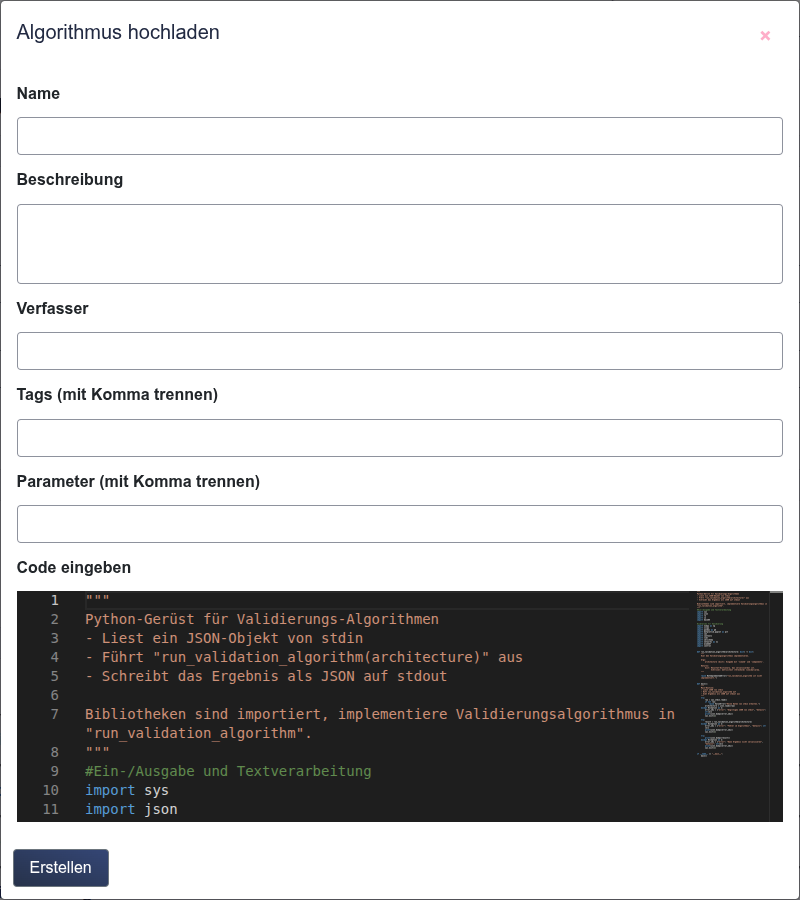
\includegraphics[width=.5\textwidth]{figures/06Evaluation/Bildschirmfoto vom 2025-08-01 11-36-46.png}
  \caption{Das Formular zum Erstellen und Hochladen des Validierungsalgorithmus}
  \label{fig:formularclean}
\end{figure}

Für diese Evaluation wird der bereits vorgestellte Traceability-Check-Algorithmus verwendet. Abbildung~\ref{fig:formularfilled} zeigt die im ArchitekturTool hinterlegten Details dieses Algorithmus, samt Beschreibung und implementierten Code.

\begin{figure}[htp!]
  \centering
  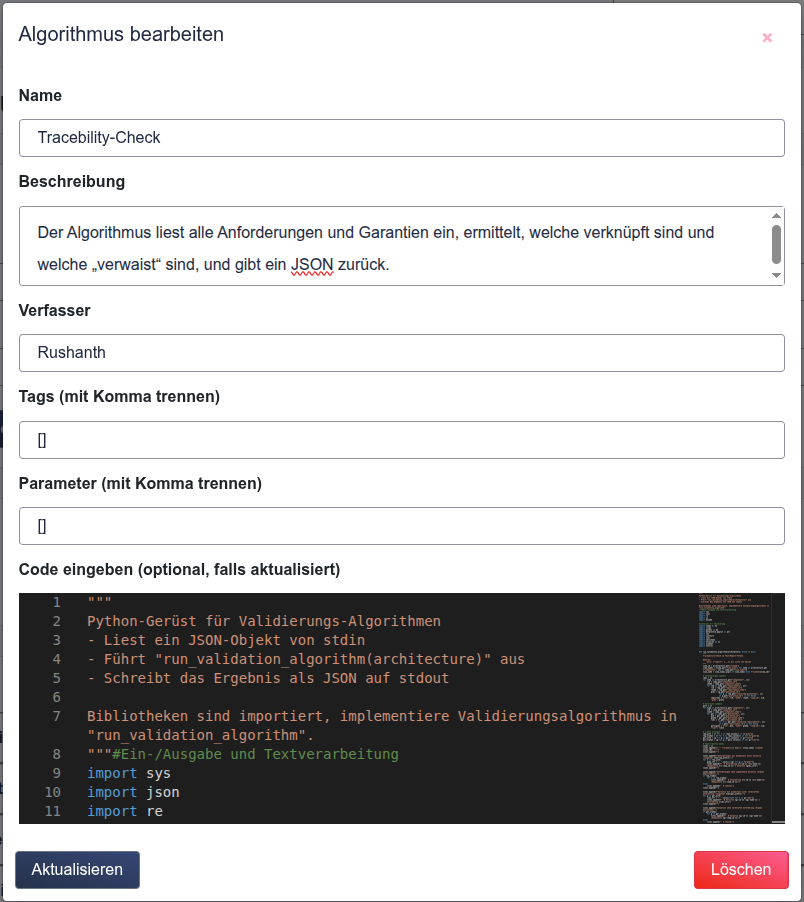
\includegraphics[width=.5\textwidth]{figures/06Evaluation/Bildschirmfoto vom 2025-08-01 11-58-21.png}
  \caption{Detailansicht des für die Evaluation genutzten Algorithmus}
  \label{fig:formularfilled}
\end{figure}

\subsection{Ausführung der Validierung und Ergebnisdarstellung}

Die Ausführung der Validierung findet in der Hauptansicht des Frameworks statt. Dafür wählt der Nutzer den gewünschten Validierungsalgorithmus, was in diesem Anwendungsbeipsiel der Traceability-Chick ist, und die zu prüfende Architektursicht aus, wie in Abbildung~\ref{fig:valstart} zu sehen.

\begin{figure}[htp!]
  \centering
  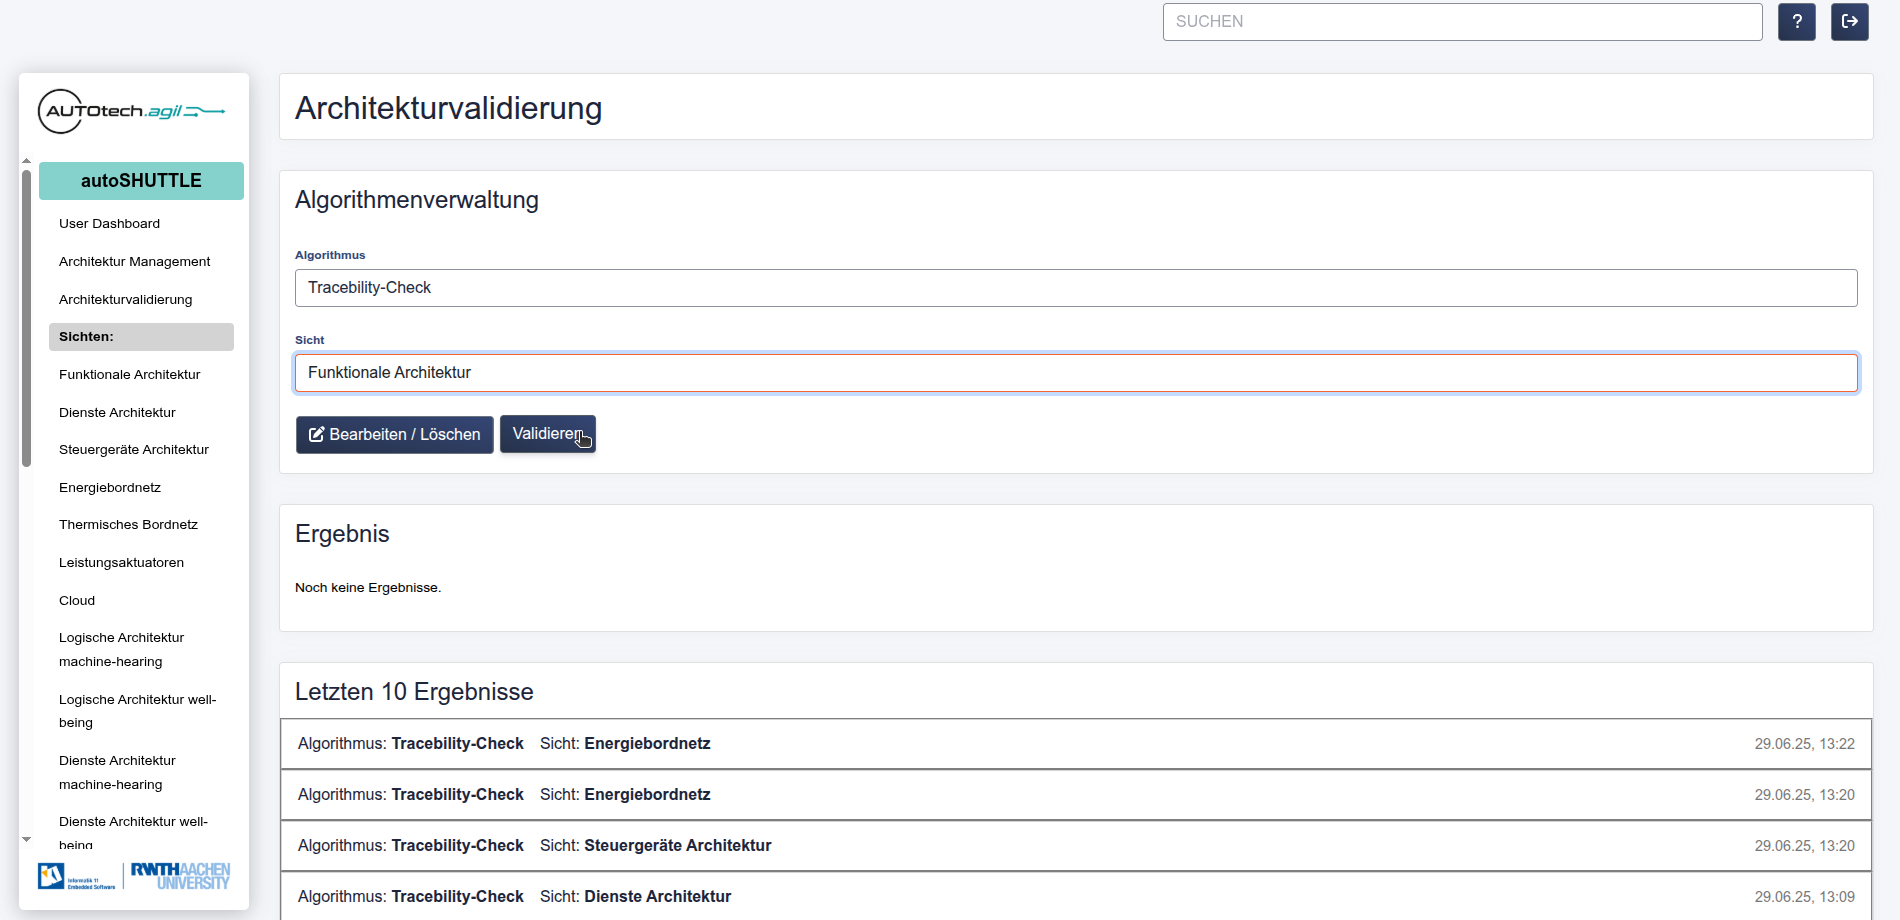
\includegraphics[width=\textwidth]{figures/06Evaluation/Bildschirmfoto vom 2025-06-30 09-16-40.png}
  \caption{Auswahl des Algorithmus und der zu validierenden Architektursicht.}
  \label{fig:valstart}
\end{figure}

Durch einen Klick auf den \glqq Validieren\grqq{}-Button wird der Prozess gestartet: Das Frontend sendet den Request über die \gls{api} an das Backend, der Algorithmus wird ausgeführt und das Ergebnis zurückgesendet.

Bei diesem Szenario wird eine Architektur verwendet, die Lücken in der Rückverfolgbarkeit enthält: Anforderungen, denen keine Garantien zugeordnet sind. Daher wird erwartet, dass der Algorithmus genau diese Anforderungen identifiziert und im Ergebnis aufzeigt.

Das Ergebnis der Ausführung ist in Abbildung~\ref{fig:valresult}, bzw. in Abbildung~\ref{fig:fullresult} ausführlich, dargestellt. Die Ausgabe entspricht den Erwartung: Der Bericht listet die Anforderungen ohne zugehörigen Garantien auf und belegt damit, dass das Framework wie gewünscht funktioniert und Lücken in der spezifizierten Architektur aufzeigen kann.

\begin{figure}[htp!]
  \centering
  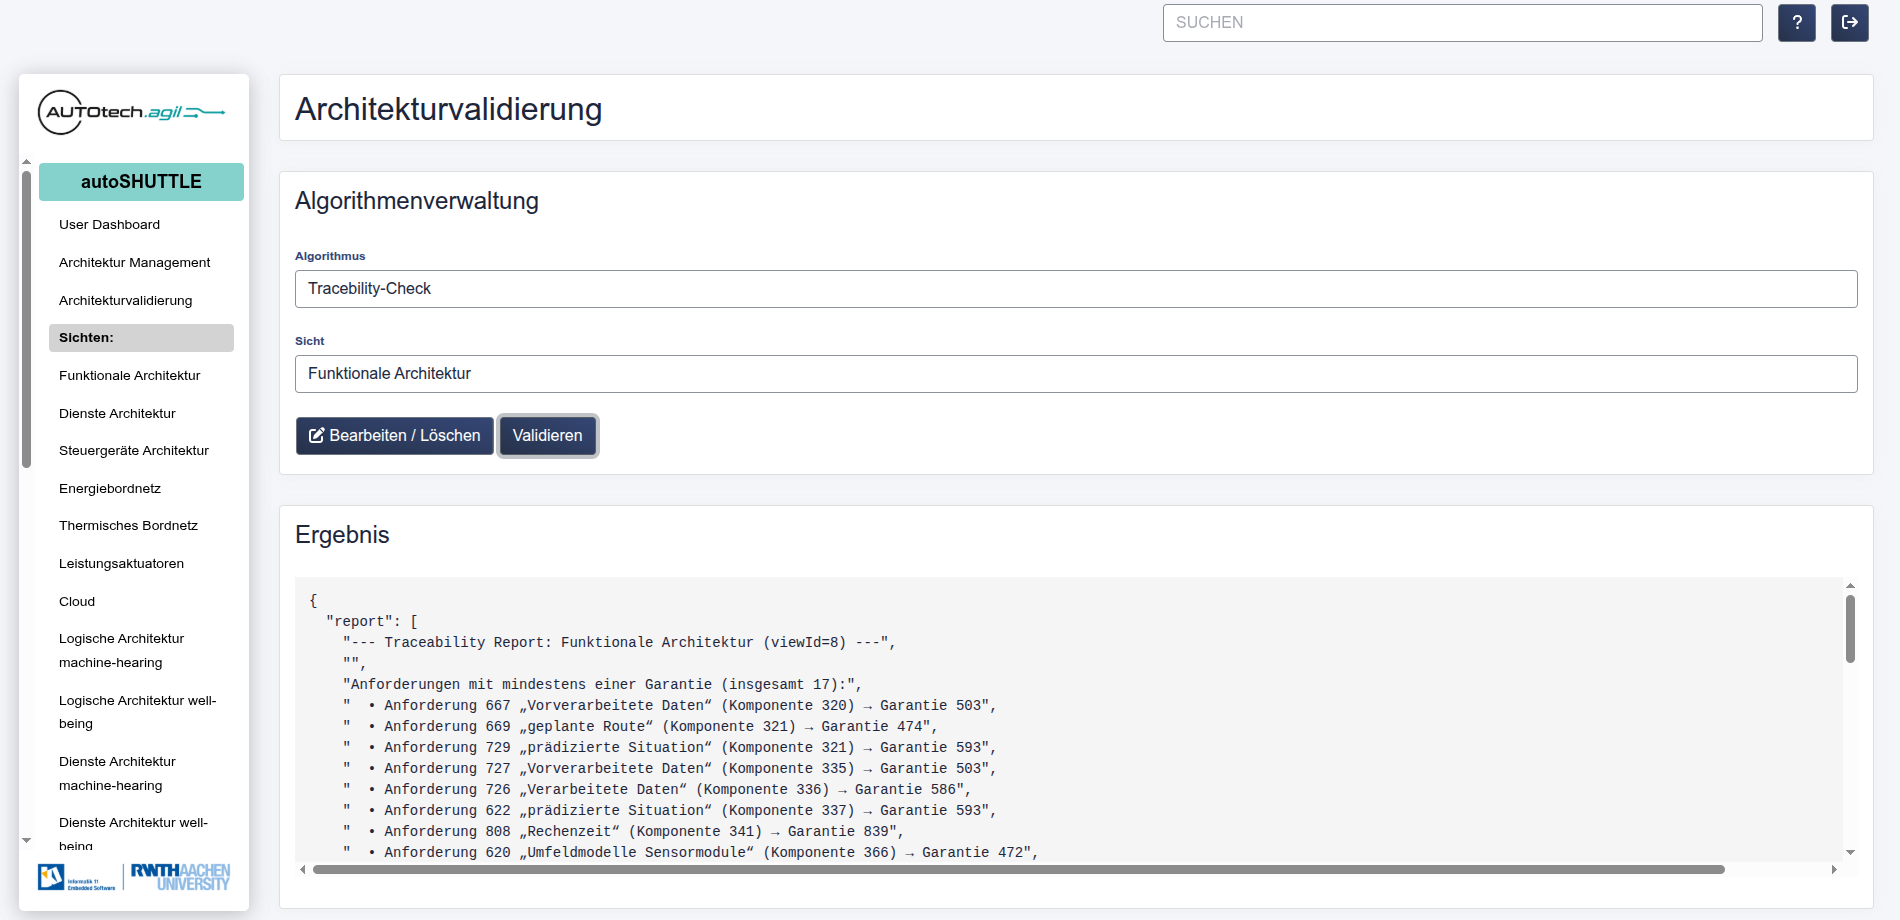
\includegraphics[width=\textwidth]{figures/06Evaluation/Bildschirmfoto vom 2025-06-30 09-17-02.png}
  \caption{Darstellung des Reports mit der korrekt identifizierten Anforderungen ohne Garantien.}
  \label{fig:valresult}
\end{figure}


\section{Bewertung der Ergebnisse}
\label{sec:analyse}

Aufbauend auf dem Nachweis aus dem vorherigen Abschnitt werden die Ergebnisse nun bewertet und eingeordnet. Es wurde gezeigt, dass das Framework den Traceability-Check-Algorithmus ausführen und dessen Ergebnisse korrekt darstellen kann. Der Fokus der folgenden Bewertung liegt darauf, diese gezeigte Funktionalität systematisch mit den initialen Anforderungen aus Abschnitt~\ref{sec:Anforderungsanalyse} abzugleichen. Damit soll klar belegt werden, dass die in der Konzeptionsphase gestellten Ziele durch die Implementierung vollständig erfüllt wurden.

Tabelle~\ref{tab:evaluationtable} fasst den Abgleich der Anforderungen mit den Evaluationsergebnissen kompakt zusammen.

\begin{table}[h!]
  \centering
  \footnotesize
  \begin{tabularx}{\textwidth}{l l l X}
    \toprule
    \textbf{ID} & \textbf{Anforderung}           & \textbf{Status} & \textbf{Begründung}                                                                                                                                                                                     \\
    \midrule                                                                                                                                                                                                                                                                 \\
    (FA-1)      & Algorithmen-API                & \checkmark      & Der erfolgreiche Durchlauf des Testszenarios belegt die funktionale Korrektheit der \gls{api}, welche die Kommmunikation zwischen Front- und Backend sicherstellt.                                      \\
    \midrule                                                                                                                                                                                                                                                                 \\
    (FA-2)      & GUI-Algorithmenverwaltung      & \checkmark      & Abbildung~\ref{fig:formularclean} bis \ref{fig:valresult} zeigt, dass die Verwaltung und die Auswahl von Validierungsalgorithmen und Architektursichten über die \gls{gui} wie gefordert möglich        \\
    \midrule                                                                                                                                                                                                                                                                 \\
    (FA-3)      & GUI-Ergebnisvisualisierung     & \checkmark      & Abbildung~\ref{fig:valresult} bzw. \ref{fig:fullresult} zeigen, dass die Ergebnis-Komponente einen textuellen Bericht wie gewünscht darstellt und somit die Anforderung an die  Visualisierung erfüllt. \\
    \midrule                                                                                                                                                                                                                                                                 \\
    (FA-4)      & Erster Validierungsalgorithmus & \checkmark      & Der Traceability-Check hat die Anforderungen ohne Garantien in der Architektur wie erwartet identifiziert und diente somit als \gls{poc} für das Framework.                                                                                                                                                                                                       \\
    \midrule                                                                                                                                                                                                                                                                 \\
    (NFA-1)     & Standardisierte API            & \checkmark      & Die in Abschnitt~\ref{subsec:api} implementierte \gls{api} folgt den Prinzipien des \gls{rest}-Standards und garantiert eine lose Koppelung.                                                                                                                                                                                                       \\
    \midrule                                                                                                                                                                                                                                                                 \\
    (NFA-2)     & Benutzerfreundlichkeit         & \checkmark      & Die klare Struktur der \gls{gui}, welche man in den Abbildung~\ref{fig:formularclean} bis \ref{fig:valresult} sehen konnte, mit getrennten Bereichen für Algorithmenverwaltung, Ergebnisdarstellung und Ergebnishistorie ermöglicht eine einfache und nachvollziehbare Bedienung.                                                                                                                                                                                                      \\
    \bottomrule
  \end{tabularx}
  \caption{Evaluation der Anforderungen}
  \label{tab:evaluationtable}
\end{table}

Die Analyse zeigt, dass alle funktionalen und nicht-funktionalen Anforderungen an das entwickelte Framework durch die Implementierung erfüllt wurden.

\section{Fazit der Evaluation}
\label{sec:fazitevaluation}

Mittels der Evaluation konnte die Funktionsfähigkeit des Framework zur automatisierten Architekturvalidierung nachgewiesen werden. Der durchgeführte \gls{poc} zeite die vollständige Ausführung von Anbindung eines Validierungsalgorithmus über dessen Ausführung auf einer im Tool spezifizierten Architektur bis hin zur korrekten Darstellung der Ergebnisse. Es wurde gezeigt, dass das Hauptziel dieser Arbeit, die automatisierte Architekturvalidierung, erreicht wurde.